\section{The SlowLab task}
\begin{figure}[t]
\centering
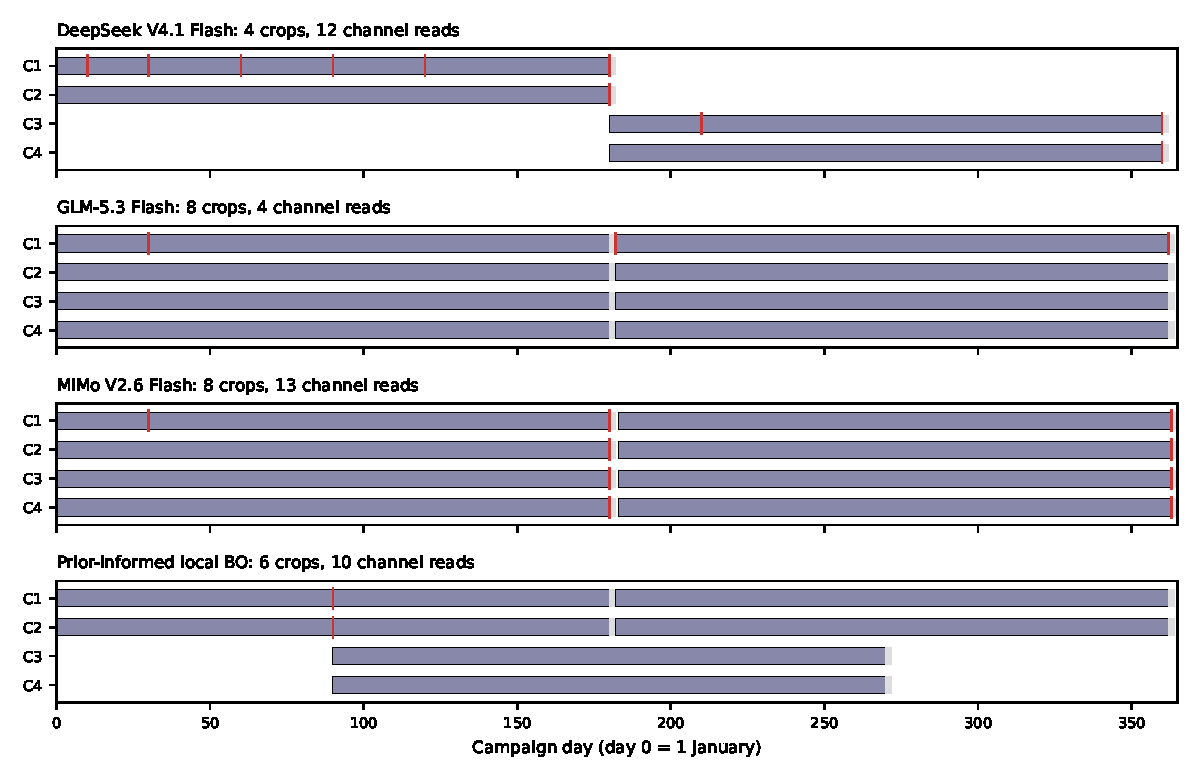
\includegraphics[width=0.9\linewidth]{figures/fig1_timelines.pdf}
\caption{Four real Full-feedback campaigns on test site 0 (selection fixed before plotting: repeat 0 of each model, seed 0 of the baseline). Bars are crops in the four compartments C1--C4 (grey: cleaning), red ticks are channel reads. Campaigns differ in how many crops they run and when; none stops a crop.}
\label{fig:timelines}
\end{figure}

\begin{table}[t]
\centering\small
\caption{The SlowLab task (contract v8, site distribution v1). ``Assumed'' marks declared assumptions without a calibration source; ``literature'' marks ranges constrained by published values.}
\label{tab:task}
\begin{tabular}{@{}p{0.2\linewidth}p{0.48\linewidth}p{0.24\linewidth}@{}}
\toprule
Element & Specification & Basis \\
\midrule
Facility & 4 independent compartments of 96~m$^2$; GreenLight \texttt{fa502ed}; Cabauw weather & simulator; audited weather \\
Calendar & 365-day campaign; crop 180 d; cleaning 2 d; last start day 183; control step 300~s & benchmark design \\
Policy & day 18--26\,$^\circ$C; night 15--22\,$^\circ$C ($\le$ day); CO$_2$ 400--1200~ppm; light 0--16~h; vent offset 2--6\,$^\circ$C; RH limit 70--90\% & design bounds \\
Actions & start, stop (crop discarded), advance, observe, recommend; analysis tools incl.\ process predictor & benchmark design \\
Observations & air temperature, RH, CO$_2$, canopy LAI proxy; cumulative harvest, heat, light, CO$_2$ dosing; every 300~s & sensor noise v0 (assumed) \\
Feedback & Full: all records at any time; Endpoint: status while running, totals at close & experimental factor (E2) \\
Budget & 16 starts; 32 decision calls; 128 tool calls; $5\times10^6$ prompt characters (models) & benchmark design \\
Score & mean margin of two crops (1 Jan, 2 Jul) in 3 new weather years, at public site prices & private evaluator \\
Site: cultivar & temperature-window shift $\pm1.5$\,$^\circ$C; photosynthesis and fruit growth $\times$0.85--1.15; earliness $\times$0.9--1.1; max LAI 2.5--3.5 & assumed \\
Site: facility & cover transmission 0.75--0.88; leakage $3\cdot10^{-5}$--$2\cdot10^{-4}$; LED efficacy 0.45--0.6 & literature \\
 & ventilation $\times$0.8--1.2; side-wall exchange 1--3~W/m$^2$K; deep soil 8--20\,$^\circ$C & assumed \\
Site: other & prices (public); unobservable per-compartment differences; campaign and evaluation years & declared \\
\bottomrule
\end{tabular}
\end{table}
\paragraph{Facility and crops.} Table~\ref{tab:task} summarises the task. Each site has four independent compartments of 96~m$^2$ simulated with the GreenLight greenhouse model \citep{katzin2020greenlight} (pinned commit \texttt{fa502ed}) under historical outdoor weather from the Cabauw observatory \citep{knmi_cabauw}. A crop runs for 180 days, after which the compartment is cleaned for 2 days; no crop may start after day 183 of the 365-day campaign. The controller acts every 300~s. Stopping a running crop discards it without salvage. Crops are stopped for safety if indoor air stays below 5\,$^\circ$C or above 40\,$^\circ$C for an hour or if they fail physiologically.

\paragraph{Policies.} A policy fixes six set-points for a whole crop: day temperature (18--26\,$^\circ$C), night temperature (15--22\,$^\circ$C, not above day), CO$_2$ target (400--1200~ppm), supplemental light (0--16~h/day), ventilation temperature offset (2--6\,$^\circ$C) and ventilation humidity threshold (70--90\%).

\paragraph{Actions, observations and budget.} The agent can start, stop, advance time, observe and recommend, and may call public analysis tools (data summaries, a Gaussian-process fit, candidate prediction and a process predictor of final crop margin trained on separate development sites). Eight channels are measured every 300~s (air temperature, humidity, CO$_2$, an image-based canopy LAI proxy with error, and cumulative harvest, heating, lighting and CO$_2$ dosing). Climate readings carry sensor error and occasional dropouts. A campaign allows at most 16 crop starts, 32 decision calls and 128 tool calls; a language-model agent may send at most $5\times10^6$ prompt characters per campaign, keeps full results only for its six most recent steps and a 2{,}000-character notebook.

\paragraph{Feedback conditions.} Under \emph{Full} feedback every record measured so far can be read at any time. Under \emph{Endpoint} feedback the agent sees only operational status while a crop runs and each crop's accrued totals when it closes.

\paragraph{Scoring.} The recommended policy is scored as the mean contribution margin per m$^2$ of two crops grown under it, one planted on 1 January and one on 2 July, averaged over three evaluation weather years not used in the campaign; this rule is public, the score is not. Margins use the site's public prices for fruit, electricity, heat and CO$_2$.

\paragraph{Sites.} A site draws cultivar parameters (temperature-window shift, photosynthetic capacity, fruit growth potential, earliness, maximum LAI), facility parameters (cover transmission, leakage, ventilation coefficient, side-wall heat exchange, LED efficacy, deep-soil temperature) and prices, plus small unobservable per-compartment differences. The distribution was fixed from physical and economic plausibility before any method was run and is never filtered on outcomes. Each site uses one campaign year and three evaluation years drawn without replacement from eleven audited formal years (2002--2011, 2015); development work used separate years and a separate master seed.
